\documentclass[10pt,letterpaper,twoside]{article}
\usepackage{code/manuscript_assets/researchpreprint}
\usepackage{amsmath,amssymb,mathtools,amsthm}
\usepackage{booktabs,graphicx}
\usepackage[hidelinks]{hyperref}
\newcommand{\norm}[1]{\left\lVert#1\right\rVert}
\newcommand{\R}{\mathbb{R}}
\newtheorem{theorem}{Theorem}

\begin{document}
\title{Variance-Weighted Residual Subspaces for Missing Ion-Resolved Readouts}
\author{Molena Huynh}
\email{molena.huynh@jmp.com}
\affiliation{North Carolina State University}

\maketitle

\begin{abstract}
Ion-resolved experiments produce short, heteroscedastic sequences for which a
missing detector interval can remove a substantial fraction of one spatial
profile. A residual-subspace reconstruction is introduced for this setting.
Complete development profiles are centered separately, their leading right
singular vectors define a spatial residual basis, and an incomplete profile is
reconstructed by variance-weighted least squares in the span of that basis and
the constant vector. A deterministic theorem separates unmodeled residual on
missing coordinates from noise amplified through the sampled basis. Exact
recovery follows when the profile lies in the learned span and the sampled
basis has full column rank. Recovery costs $O(n_o r^2+r^3+nr)$ operations and
stores $nr$ basis scalars. Evaluation uses 561 authenticated site-resolved
averages from a 51-ion experiment, each derived from 1000 shots. Seven early
times select $r=4$ by leave-one-time-out reconstruction; times 8--10 ms remain
untouched for confirmation. Across periodic one-in-five losses and five
contiguous ten-ion outages, confirmation RMSE is 0.06270, compared with
0.08435 for the strongest simple comparator. This is a 44.7 percent reduction
in pooled squared error. The method wins 25 of 30 mask--time cases; all five
losses and the complete rank sensitivity are reported. The result supports a
compact readout-recovery primitive, not universal dominance or a microscopic
dynamical model.
\end{abstract}

\section{Ion-resolved recovery problem}

Consider a measured profile $x\in\R^n$ with observed coordinate set
$\Omega$ and missing set $\Gamma$. Coordinate restrictions are denoted by
$P_\Omega$ and $P_\Gamma$. The data in this study are staggered-spin averages
from a 51-ion N\'eel-state experiment~\cite{joshi2025data,kraft2025beqs}.
The archive contains eleven times and 51 sites, with a reported standard error
for every average. Missing-coordinate recovery differs from forecasting:
measurements at the retained sites of the current time are available, while a
periodic detector loss or contiguous outage hides the remaining sites.

Spatial interpolation assumes local smoothness. That assumption is poorly
matched to the alternating and boundary-dependent residuals in the measured
profiles. A constant fill discards persistent spatial structure. The method
below retains a constant component for the instantaneous global level and
learns only the spatial residual directions from earlier complete profiles.
This separation prevents the dominant temporal oscillation from consuming the
limited rank.

\section{Variance-weighted residual subspace}

Let $X\in\R^{T\times n}$ contain complete development profiles. Define
\begin{equation}
 R=X-\operatorname{diag}(X\mathbf 1/n)\mathbf 1^T,
 \qquad R=Q\Sigma V^T,
 \label{eq:residual-svd}
\end{equation}
and let $U=V_{:,1:r}$. The reconstruction design is
$A=[\mathbf 1\;U]\in\R^{n\times(r+1)}$. If $s_i$ is the reported standard
error, the observed-coordinate weight is
$W=\operatorname{diag}(1/\max\{s_i,10^{-2}\})_{i\in\Omega}$.
The coefficient and reconstructed profile are
\begin{align}
 \widehat z
 &=\arg\min_{z\in\R^{r+1}}
   \norm{W(P_\Omega Az-P_\Omega x)}_2^2
   +\lambda\norm{z_{2:r+1}}_2^2,
 \label{eq:objective}\\
 \widehat x&=A\widehat z. \label{eq:reconstruction}
\end{align}
The registered grid contains $r=1,\ldots,7$ and $\lambda=0$; the latter is
fixed because every development sampled design is well conditioned at the
candidate ranks. Ties are resolved toward smaller rank.

\begin{theorem}[Missing-coordinate error]
\label{thm:error}
Assume $\lambda=0$ and $M=WP_\Omega A$ has full column rank. For every
$x=Az_\star+e$,
\begin{equation}
 \norm{P_\Gamma(\widehat x-x)}_2
 \le \norm{P_\Gamma e}_2
 +\frac{\norm{P_\Gamma A}_2}{\sigma_{\min}(M)}
       \norm{WP_\Omega e}_2 .
 \label{eq:bound}
\end{equation}
In particular, $e=0$ implies $\widehat x=x$.
\end{theorem}

\begin{proof}
Substitution of $P_\Omega x=P_\Omega Az_\star+P_\Omega e$ into the
full-rank weighted least-squares solution gives
\begin{equation}
 \widehat z=M^\dagger WP_\Omega x
 =z_\star+M^\dagger WP_\Omega e. \label{eq:coefficient-error}
\end{equation}
Consequently,
\begin{equation}
 P_\Gamma(\widehat x-x)
 =P_\Gamma A M^\dagger WP_\Omega e-P_\Gamma e.
\end{equation}
The triangle inequality, submultiplicativity, and
$\norm{M^\dagger}_2=1/\sigma_{\min}(M)$ prove Eq.~\eqref{eq:bound}.
When $e=0$, Eq.~\eqref{eq:coefficient-error} gives
$\widehat z=z_\star$ and hence exact recovery.
\end{proof}

The two terms in Eq.~\eqref{eq:bound} expose distinct limitations. The first
is residual structure absent from the learned span on the missing sites. The
second is observed residual amplified by poor sampling of the basis. Thus a
larger rank can reduce approximation error while decreasing
$\sigma_{\min}(M)$, an effect measured directly in the rank experiment.

\begin{theorem}[Arithmetic and storage]
\label{thm:complexity}
Given $U$, one reconstruction with $n_o=|\Omega|$ and rank $r$ uses
$O(n_or^2+r^3+nr)$ arithmetic and $O(nr+r^2)$ auxiliary storage. The stored
model contains exactly $nr$ basis scalars in addition to singular values.
\end{theorem}

\begin{proof}
Forming the weighted normal matrix and right-hand side costs
$O(n_or^2)$. Factoring the $(r+1)$-dimensional normal matrix costs $O(r^3)$,
and applying $A$ costs $O(nr)$. The basis and normal matrix occupy $nr$ and
$O(r^2)$ scalars, respectively. No $n\times n$ matrix is formed.
\end{proof}

\section{Registered experimental design}

The source archive and license are recorded in Table~\ref{tab:data}. Times
1--7 ms form development cases. Each development time is omitted in turn from
the basis construction, preventing its hidden entries from influencing rank
selection. After selecting the rank, times 0--7 ms form the fixed basis for
confirmation at 8--10 ms. The two mask families contain five offsets each:
periodic removal of one site in five and contiguous removal of ten sites. The
resulting confirmation set contains 30 mask--time cases.

\begin{table}[b]
\caption{Authenticated data and fixed evaluation protocol.}
\label{tab:data}
\begin{ruledtabular}
\begin{tabular}{lc}
Quantity & Value\\ \hline
Source & Zenodo 10.5281/zenodo.17750419\\
License & CC BY 4.0\\
Ion-resolved averages & 561\\
Shots per time & 1000\\
Development times & 1--7 ms\\
Confirmation times & 8--10 ms\\
Candidate ranks & 1--7\\
Selected rank & 4\\
Confirmation cases & 30
\end{tabular}
\end{ruledtabular}
\end{table}

Comparators use only the retained coordinates of the current profile. They
are the observed-site mean, piecewise-linear spatial interpolation, and
nearest-site fill. RMSE is computed only on hidden coordinates. Pooled RMSE
is the square root of mean squared error over the registered cases; paired
wins are counted at the mask--time level.

\begin{figure}[t]
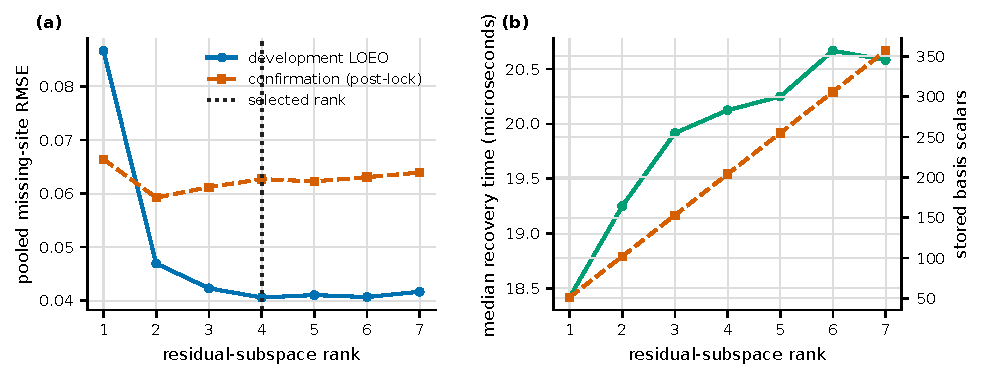
\includegraphics[width=\textwidth]{code/manuscript_assets/figures/recovery/selection_cost.pdf}
\caption{Statistical and computational rank paths. (a) Early-time
leave-one-out selection and post-lock confirmation sensitivity. Rank four
minimizes the development curve; the confirmation curve is not a selection
criterion. (b) Measured recovery time and exact basis storage. Timings are
medians of 101 runs on the stated local CPU environment.}
\label{fig:rank}
\end{figure}

\section{Results}

Figure~\ref{fig:rank} shows the complete rank path. The minimum of the
development curve occurs at $r=4$. Confirmation also remains below the
strongest simple comparator throughout the registered rank range, while its
minimum at rank two is not used for model selection.

\begin{table}[t]
\caption{Pooled confirmation error on 30 mask--time cases. The squared-error
reduction is measured against the observed-site mean, the strongest simple
comparator.}
\label{tab:results}
\begin{ruledtabular}
\begin{tabular}{lc}
Method & Missing-site RMSE\\ \hline
Residual subspace, $r=4$ & 0.06270\\
Observed-site mean & 0.08435\\
Linear interpolation & 0.12071\\
Nearest-site fill & 0.12424\\ \hline
Squared-error reduction & 44.7\%\\
Paired wins vs. mean & 25 of 30
\end{tabular}
\end{ruledtabular}
\end{table}

Table~\ref{tab:results} gives the registered aggregate. The improvement is
not uniform. Figure~\ref{fig:confirmation}(a) displays every confirmation case
and marks each loss, preventing the pooled statistic from hiding five adverse
cases. The contiguous 21--30 outage at 10 ms in
Fig.~\ref{fig:confirmation}(b) illustrates the mechanism: retained sites
determine the instantaneous offset and four development residual directions
interpolate a nonlocal spatial pattern.

\begin{figure}[t]
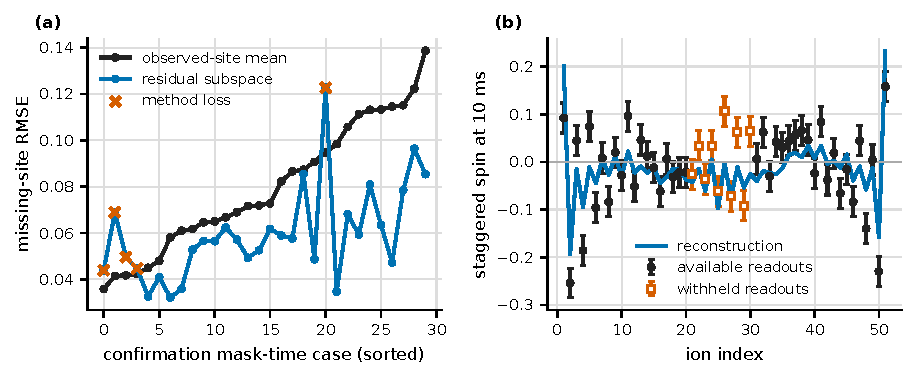
\includegraphics[width=\textwidth]{code/manuscript_assets/figures/recovery/confirmation_overview.pdf}
\caption{Confirmation evidence. (a) All 30 cases, ordered by observed-mean
error; crosses identify the five method losses. (b) A registered ten-site
contiguous outage at 10 ms. Filled circles are available measurements, open
squares are withheld measurements, and the line is the reconstruction.
Error bars are reported standard errors.}
\label{fig:confirmation}
\end{figure}

Figure~\ref{fig:rank}(b) connects the measured cost to
Theorem~\ref{thm:complexity}. Storage grows exactly as $51r$ scalars. The small
timing scale reflects this data set; the operation count, rather than a
single-device measurement, determines extrapolation to larger arrays.

\section{Scope}

Residual-subspace recovery exploits repeated spatial structure but does not
identify a Hamiltonian, Lindbladian, or measurement-noise mechanism. The
experiment contains one 51-ion sequence and three confirmation times.
Additional devices, calibrations, and independently acquired sequences are
required before attributing broad physical generality. Within the fixed
protocol, the main empirical conclusion is narrower: early-time residual
directions improve pooled missing-site recovery over three simple spatial
fills, with five explicitly reported confirmation losses.

The implementation stores no square spatial operator. Every result table and
plot is regenerated from the attributed CSV records, the registered masks,
and a deterministic rank-selection rule. The theorem supplies the associated
conditioning diagnosis: missing residual energy and sampled-basis
conditioning, rather than visual smoothness, govern reconstruction accuracy.

\bibliographystyle{plainnat}
\bibliography{code/manuscript_assets/references}
\end{document}
